光与原子相互作用的一般哈密顿量为:
\[H=H_{atom}+H_{int}\]
其中相互作用部分是电磁场与电偶极子相互作用的哈密顿量:
\[H_{int}=-\hat{E}(0,t)\cdot \hat{d}\]
其中我们可以将偶极子算符用原子态展开:
\[\hat{d}=\sum_{m,n}d_{m,n}\diracr{m}\diracl{n}=\sum_{m>n}d_{m,n}\diracr{m}\diracl{n}+h.c\]
因此相互作用表象下的偶极子算符为:
\[\hat{d}_I=e^{\frac{iH_at}{\hbar}}\hat{d}e^{\frac{-iH_at}{\hbar}}=\sum_{m>n}d_{m,n}e^{i\omega_{m,n}t}\diracr{m}\diracl{n}\]
一般在相互作用表象下处理问题,即:
\[\diracr{\Psi(t)}_I=e^{\frac{iH_at}{\hbar}}\diracr{\Psi(t)}_s\]
其中假设系统的电磁场部分不会被相互作用扰动,也就是说,态的演化为:
\[\prod_{\alpha}D(\alpha)\diracr{V}\otimes\diracr{\Psi(0)}\rightarrow\prod_{\alpha}D(\alpha)\diracr{V}\otimes\diracr{\Psi(t)}\]
由于电磁场部分波函数不会被相互作用扰动因此我们可以利用电场的期待值取代电场算符:
\[\hat{E}(r,t)=\sum_k \epsilon_k a_ke^{-i\omega_kt}+h.c\rightarrow E(r,t)=\sum_k \epsilon_k \alpha_ke^{-i\omega_kt}+c.c\]
而且光场一般都会外加强光与原子相互作用,这是一个单频光,因此我们可以忽略掉真空中光场的其他模式,只保留我们关注的模式:
\[E(r,t)=\frac{1}{2}\epsilon(t)e^{-i\omega t}+c.c\]
这里我们把其他与频率无关的因此全部放进了$\epsilon_k(t)$.从而可以得到我们需要的相互作用表象下的哈密顿量。
\begin{align}
\notag H&=\sum_{g,e}\frac{\epsilon(t)}{2}\cdot d_{eg}e^{-i(\omega-\omega_{eg})t}\diracr{e}\diracl{g}+h.c\\
&+\sum_{g,e}\frac{\epsilon^*(t)}{2}\cdot d_{eg}e^{i(\omega+\omega_{eg})t}\diracr{e}\diracl{g}+h.c
\end{align}
这时这个哈密顿量来演化我们需要的原子态。其中:
\[\omega_{eg}=\omega_e-\omega_g>0\]
例如,假设原子初始处于基态,而后演化过程中变到基态与激发态的叠加态:
\[\diracr{\Psi(0)}=\diracr{g}\]
\[\diracr{\Psi(t)}=c_e\diracr{e}+c_g\diracr{g}\]
那么由薛定谔方程我们可以得到:
\begin{align*}
&i\hbar\partial_t\diracr{\Psi(t)}=H\diracr{\Psi(t)}\\
&\rightarrow i\hbar(\dot{c}_e\diracr{e}+\dot{c}_g\diracr{g}=(\frac{\epsilon(t)}{2}\cdot d_{eg}e^{-i(\omega-\omega_{eg})t}+\frac{\epsilon^*(t)}{2}\cdot d_{eg}e^{i(\omega+\omega_{eg})t})c_g\diracr{e}+\cdots
\end{align*}
与$c_e$相关的方程为(取$c_g=1$):
\[i\hbar\dot{c}_e=(\frac{\epsilon(t)}{2}\cdot d_{eg}e^{-i(\omega-\omega_{eg})t}+\frac{\epsilon^*(t)}{2}\cdot d_{eg}e^{i(\omega+\omega_{eg})t})\]
从而可以得到:
\[c_e=\int_{0}^t\frac{\Omega_{eg}(t)}{2i}e^{i\Delta_{eg}t}dt+\int_{0}^t\frac{\Omega^*_{eg}(t)}{2i}e^{i(\omega+\omega_{eg})t}dt\]
其中我们有拉比震荡频率:
\[\Omega_{eg}=\frac{\epsilon(t)\cdot d_{eg}}{\hbar}\]
以及:
\[\Delta_{eg}=\omega_{eg}-\omega\]
$c_e$的解中第二项由于$\omega+\omega_{eg}$很大,因此积分贡献远小于第一项,从而可以忽略,等价的,也就是说哈密顿量中可以将含指数因子:
\[e^{i(\omega+\omega_{eg})t}\]
的项丢掉(Rotation Wave Approximation),因为这个震荡太快,对于缓变的系统积分后结果出来delta函数或为零,没有意义。\par
从而我们可以将哈密顿量直接写为:
\begin{align}
H_{R.W.A}&=\sum_{g,e}\frac{\hbar\Omega_{eg}(t)}{2}e^{i\Delta_{eg}t}\diracr{e}\diracl{g}+h.c\\
\notag &=\sum_{g,e}\frac{\hbar\Omega_{eg}}{2}e^{i\Delta_{eg}t}\diracr{e}\diracl{g}+h.c
\end{align}
可以再对这个系统做一个旋转波变换将时间依赖去掉,为此我们考虑一般的薛定谔方程
\[i\hbar \partial_t \Psi=H\Psi\]
假设将态做变换
\[\Psi(t)=U(t)\Psi'(t)\]
那么有:
\[i\hbar[(\partial_t U(t))\Psi'(t)+U(t)\partial_t \Psi'(t)=HU(t)\Psi'(t)\]
那么关于$\Psi'(t)$的薛定谔方程为:
\[i\hbar\partial_t\Psi'(t)=U^{-1}(t)HU(t)-i\hbar U^{-1}\partial_t U(t)\]
也就是说:
\[H'=U^{-1}(t)HU(t)-i\hbar U^{-1}\partial_t U(t)\]
对于本问题,我们可以取:
\[U=e^{i\Delta\diracr{e}\diracl{e}t}\]
这时我们有态的变化为:
\[\Psi'=U^{-1}\Psi,\diracr{e}\rightarrow e^{-i\Delta t}\diracr{e},\diracr{g}\rightarrow \diracr{g}\]
那么我们有:
\begin{align*}
U^{-1}e^{i\Delta t}\diracr{e}\diracl{g}U&=e^{-i\Delta\diracr{e}\diracl{e}t}e^{i\Delta t}\diracr{e}\diracl{g}e^{i\Delta\diracr{e}\diracl{e}t}\\
&=e^{-i\Delta t}e^{i\Delta t}\diracr{e}\diracl{g}
=\diracr{e}\diracl{g}
\end{align*}
因而消除了时间依赖因子,另一方面我们有:
\[-i\hbar U^{-1}\partial_t U(t)=-i\hbar(i\Delta \diracr{e}\diracl{e})=\hbar\Delta \diracr{e}\diracl{e}\]
因此我们最后得到做完旋转波变换后的哈密顿量为:
\[H'=\frac{\hbar\Omega_{eg}}{2}\diracr{e}\diracl{g}+\hbar\Delta_{eg} \diracr{e}\diracl{e}\]
类似的如果原始哈密顿量为:
\[H=\frac{\hbar\Omega}{2}e^{i\Delta t}\diracr{g}\diracl{e}\]
那么我们可以取:
\[U=e^{i\Delta\diracr{g}\diracl{g}t}\]
同样计算得到:
\[U^{-1}e^{i\Delta t}\diracr{g}\diracl{e}U=\diracr{g}\diracl{e}\]
\[-i\hbar U^{-1}\partial_t U(t)=\hbar\Delta \diracr{g}\diracl{g}\]
从而哈密顿量变为:
\[H'=\frac{\hbar\Omega}{2}\diracr{g}\diracl{e}+\hbar\Delta \diracr{g}\diracl{g}\]
受激震荡过程的能量关系可用能级图描述,如图\ref{fig:shouji}所示:
\begin{figure}
\begin{center}
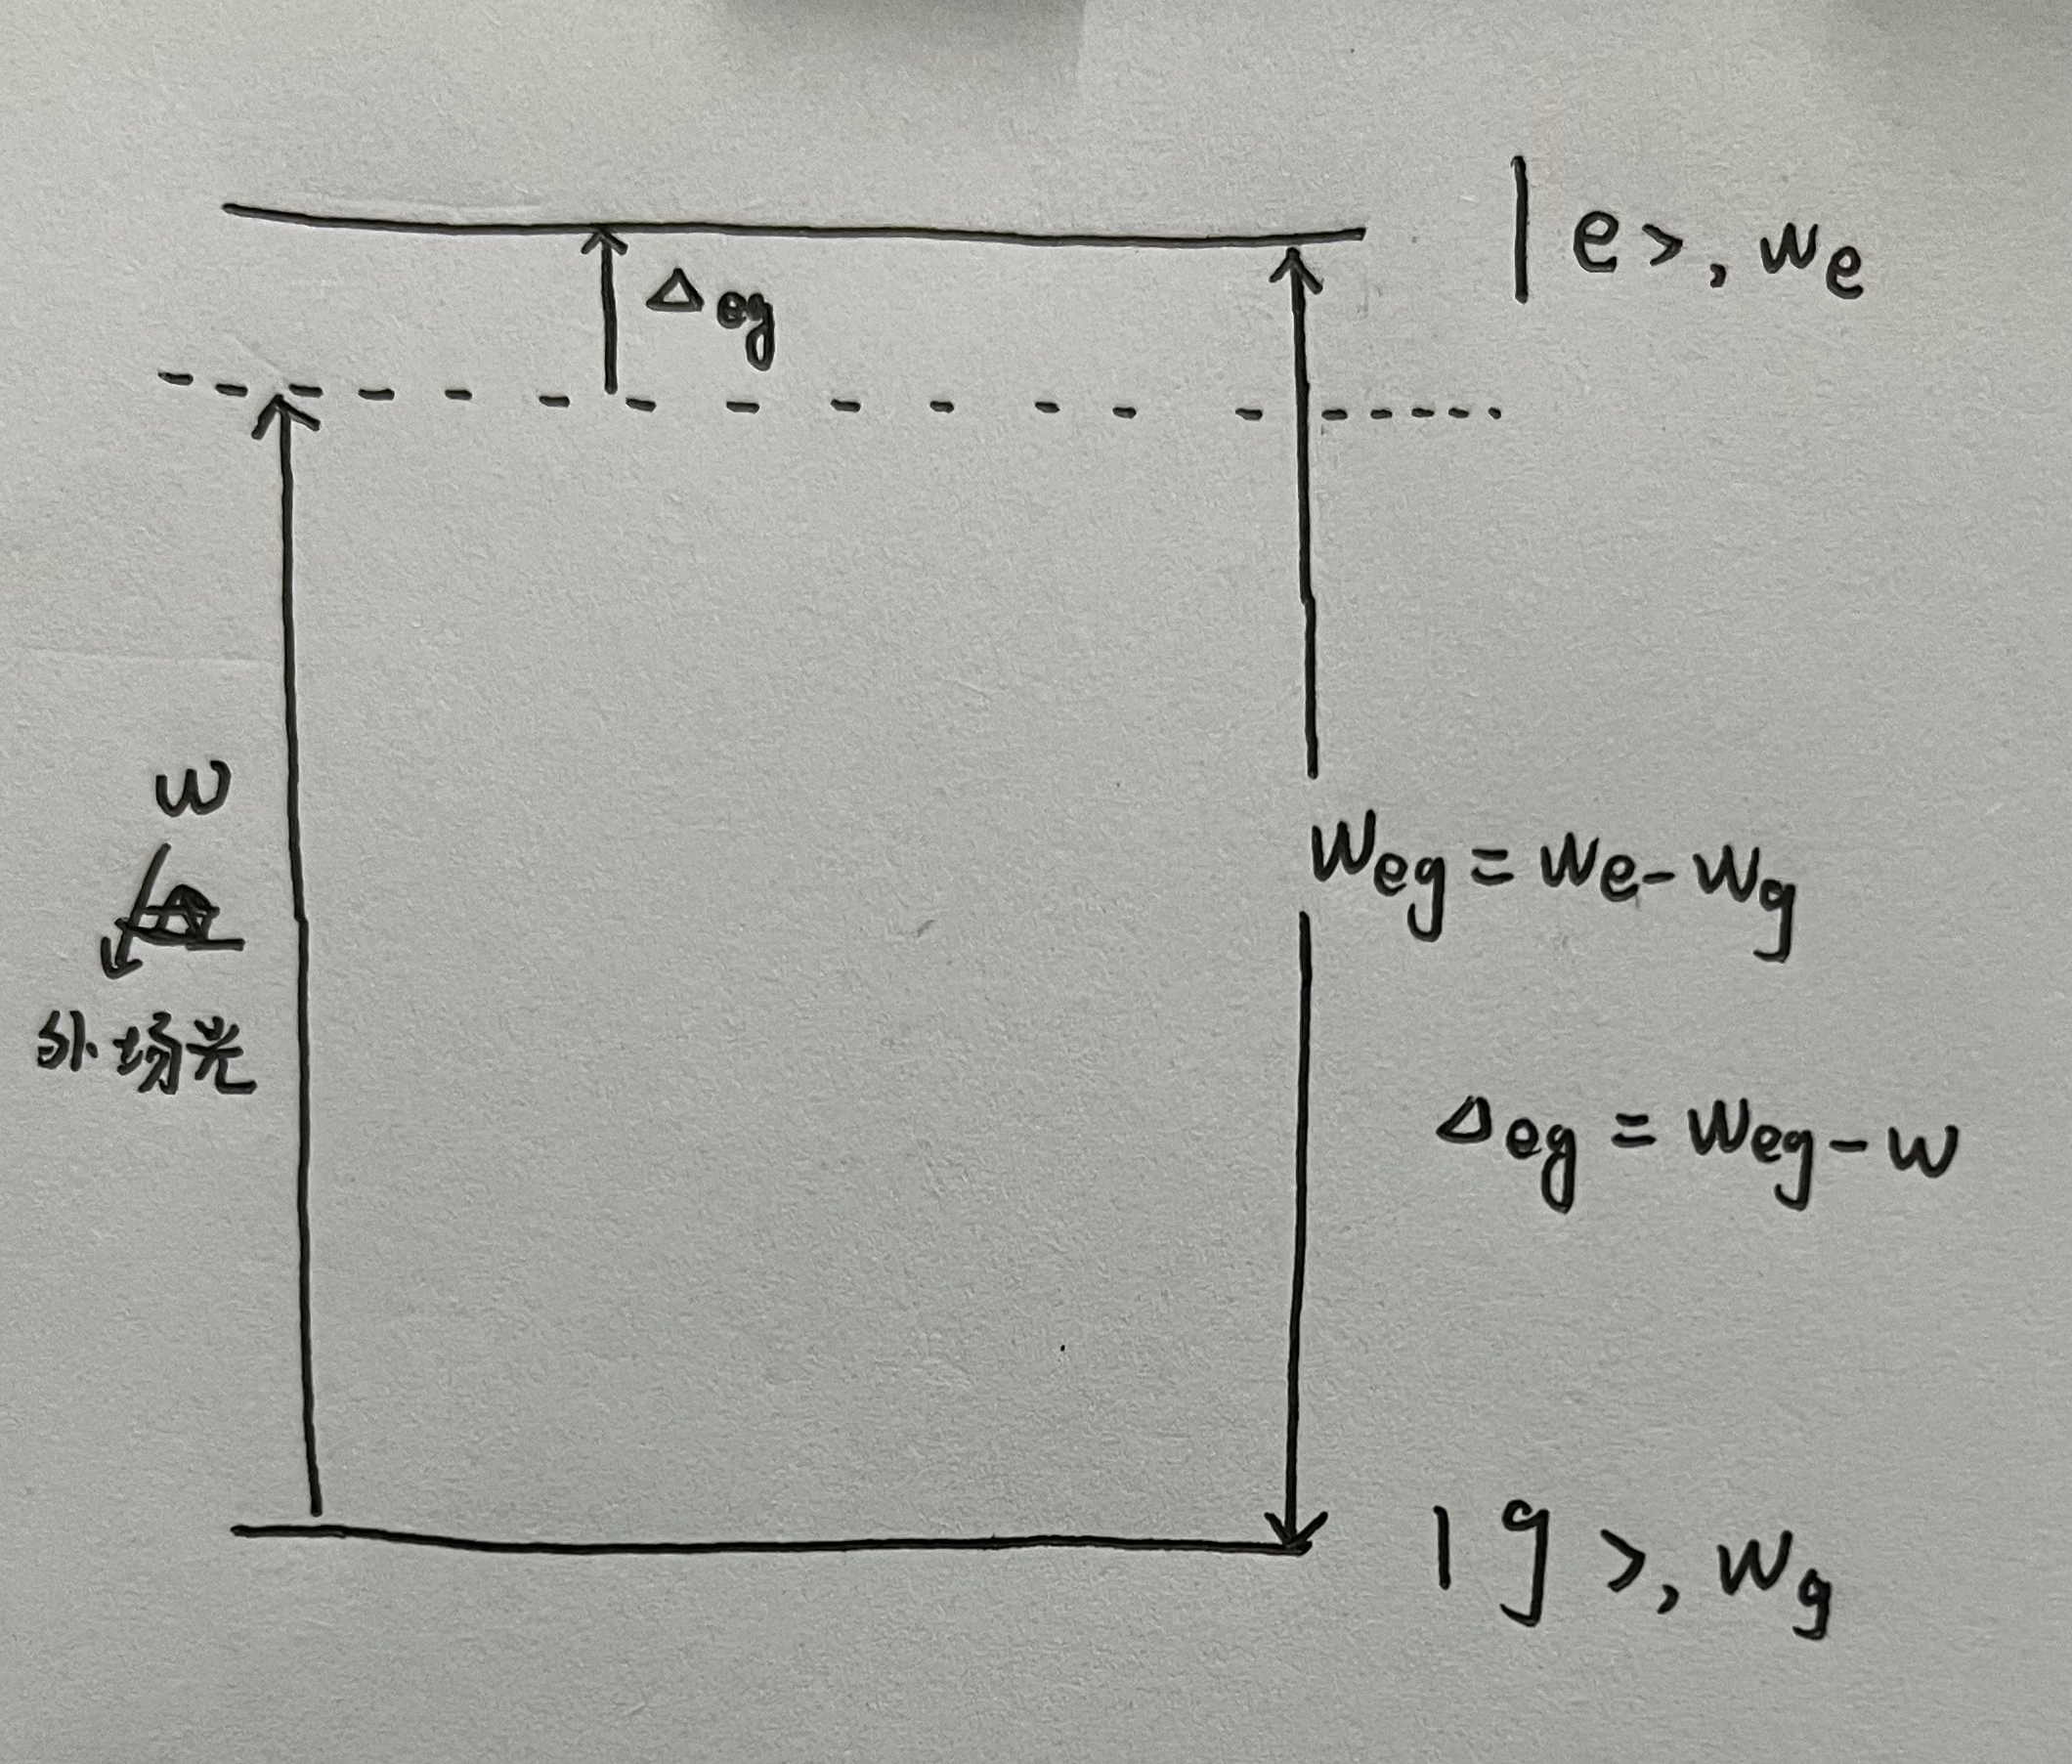
\includegraphics[height=6cm]{./figures/shouji.jpg}
\caption{受激发震荡过程的能量关系图}
\label{fig:shouji}
\end{center}
\end{figure}
可以选取基态能量为$-\frac{1}{2}\hbar\Delta$,那么我们就可以将哈密顿量写为:
\[H=\frac{1}{2}\hbar\Delta(\diracr{e}\diracl{e}-\diracr{g}\diracl{g})+\frac{\hbar\Omega}{2}\diracr{g}\diracl{e}+\frac{\hbar\Omega^*}{2}\diracr{e}\diracl{g}\]
引入pauli矩阵,那么就有:
\[H=\frac{\hbar}{2}\vec{\Omega}\cdot\vec{\sigma}\]

\subsection{bloch representation}
如果定义$\vec{\sigma}_u=\sigma\cdot u$,其中$(u=(\sin\theta\cos\phi,\sin\theta\sin\phi,\cos\theta))$
那么我们有
\[\diracr{+}_u=\cos\frac{\theta}{2}e^{-i\frac{\phi}{2}}\diracr{+}+\sin\frac{\theta}{2}e^{i\frac{\phi}{2}}\diracr{-}\]
\[\diracr{-}_u=-\sin\frac{\theta}{2}e^{-i\frac{\phi}{2}}\diracr{+}+\cos\frac{\theta}{2}e^{i\frac{\phi}{2}}\diracr{-}\]
定义一般的态$\diracr{\Psi(\theta,\phi)}=\diracr{+}_u$,那么我们有密度矩阵:
\[\rho=\frac{1}{2}(1+\vec{u}\cdot \vec{\sigma})\]
那么我们可以得到这个一般的态在哈密顿量为
\[H=\frac{\hbar}{2}\vec{\Omega}\cdot\vec{\sigma}\]
演化下的运动方程变为:
\[\dot{u}=\Omega\times u\]